\documentclass[aspectratio=169]{beamer}

% ============================================================
% University of Toronto brand palette (official colors)
% ============================================================
\usepackage{xcolor}
\definecolor{UofTBlue}{HTML}{1E3765}      % primary — Pantone 655
\definecolor{BoundlessBlue}{HTML}{007FA3} % secondary — Pantone 633
\definecolor{UofTGrey}{HTML}{F2F4F7}      % backgrounds only
\definecolor{UofTBlack}{HTML}{000000}

\usetheme{default}
\setbeamercolor{structure}{fg=UofTBlue}
\setbeamercolor{title}{fg=UofTBlue}
\setbeamercolor{frametitle}{fg=UofTBlue,bg=UofTGrey}
\setbeamercolor{section in toc}{fg=UofTBlue}
\setbeamercolor{block title}{fg=white,bg=UofTBlue}
\setbeamercolor{block body}{fg=UofTBlack,bg=UofTGrey}
\setbeamercolor{alerted text}{fg=BoundlessBlue}
\setbeamertemplate{navigation symbols}{}
\setbeamertemplate{footline}[frame number]

% Trade Gothic/Bembo (official UofT type) require a commercial license.
% Fira Sans is a reasonable free stand-in for headings if available;
% falls back to the beamer default cleanly if not installed.
\IfFileExists{FiraSans.sty}{\usepackage[sfdefault]{FiraSans}}{}

\usepackage{amsmath,amssymb,amsthm,mathtools}
\usepackage{stmaryrd} % \llbracket, \rrbracket — needed for \Brack
\usepackage{tikz}
\usepackage{booktabs}
\usepackage{graphicx}
\usepackage{subcaption}
\usepackage{appendixnumberbeamer} % freezes the footline frame counter at \appendix,
                                   % so backup slides all show the same "N/N" as the
                                   % last main-talk slide instead of continuing to count up
\usepackage{pdfpages} % for borrowing pages verbatim from 2023 UTMUST - Easy to solve.pdf

% Tikz styles/libraries, copied verbatim from common/tonas-thesis.sty so
% that \input-ing figures straight from the thesis (figures/*.tex) renders
% correctly without redefining anything.
\usetikzlibrary{positioning, arrows.meta, shapes.geometric, calc, decorations.markings, decorations.pathmorphing, decorations.pathreplacing}
\tikzset{
    vertex/.style={circle, draw, fill=black, inner sep=0pt, minimum size=4pt},
    vlabel/.style={font=\small, color=black},
    dot/.style={circle, fill=black, inner sep=0pt, minimum size=3pt, anchor=center},
    arrow/.style={-{Latex[length=3pt, width=2.5pt]}, thin, black!60}
}

% ============================================================
% Notation macros, copied verbatim from the thesis's shared preamble
% common/tonas-thesis.sty (the \DeclareMathOperator / \newcommand
% block only — NOT the full package, which also redefines \newtheorem
% environments with [chapter]-numbering that presupposes a \chapter
% counter beamer does not have and would break compilation).
% Source: common/tonas-thesis.sty, "Common Operators" section.
% ============================================================
\DeclareMathOperator{\Fer}{Fer}
\DeclareMathOperator{\Aut}{Aut}
\DeclareMathOperator{\Stab}{Stab}
\DeclareMathOperator{\dom}{dom}
\DeclareMathOperator{\img}{img}
\DeclareMathOperator{\bal}{bal}
\DeclareMathOperator{\Hom}{Hom}
\DeclareMathOperator{\cl}{cl}
\DeclareMathOperator{\id}{id}
\DeclareMathOperator{\tp}{tp}
\DeclareMathOperator{\ex}{ex}
\renewcommand{\restriction}{\mathord{\upharpoonright}}
\newcommand{\tFer}{\texttt{Fer}\ }
\newcommand{\tfer}{\texttt{fer}\ }
\newcommand{\len}{\mathrm{len}}
\newcommand{\RecFer}{\texttt{RecFer}}
\newcommand{\NN}{\mathcal{N}}
\newcommand{\CC}{\mathcal{C}}
\newcommand{\DD}{\mathcal{D}}
\newcommand{\CF}{\mathcal{C}_F}
\newcommand{\Brack}[1]{\left\llbracket{#1}\right\rrbracket}
\newcommand{\Cp}{\mathrm{C}_{\mathrm{p}}}
\newcommand{\hatC}{\hat{\mathbb{C}}}

\title{On Complexity, Computation, and Graph Homomorphisms}
\subtitle{PhD Thesis Defence}
\author{Tonatiuh Matos Wiederhold}
\institute{Department of Mathematics, University of Toronto \\ Advisors: Spencer Unger, Franklin D. Tall}
\date{July 27, 2026}

\begin{document}

\begin{frame}
  \titlepage
\end{frame}

\begin{frame}{Outline}
  \tableofcontents
\end{frame}

\begin{frame}{Publications}
  \scriptsize
  \begin{tabular}{@{}p{3.3cm}p{8.4cm}@{}}
    \toprule
    \textbf{Thesis section} & \textbf{Basis} \\
    \midrule
    \S2.3 Dichromatic number & Sole-authored; Caltech Logic Seminar (Apr.\ 2026); arXiv (2026) \\
    \S2.4 Cantor game & Matos-Wiederhold--Salvetti, \emph{Topology Proceedings} (2025) \\
    \S3.x Deep Computations & Due\~nez--Iovino--Matos-Wiederhold--Salvetti--Tall, arXiv (2026) \\
    \S4.2 Border tracing & P.~Wiederhold--Matos-Wiederhold, \emph{Theoretical Comp.\ Science} (2026) \\
    \S4.3 Recursive constructions & Eslava et al., \emph{Aequationes Mathematicae} (2025) \& Caro et al., \emph{Procedia Computer Science} (2023) \\
    \bottomrule
  \end{tabular}
\end{frame}

% Borrowed from the 2023 UTMUST outreach talk "Easy to solve, impossible to
% describe" --- the circle-colouring example illustrating the same
% easy/computable/definable trade-off the thesis is about. Pages come in
% verbatim (original PowerPoint styling, not UofT-themed) at full vector
% quality since the source is already 16:9.
\includepdf[pages={3,6,12,16,22},width=\paperwidth,pagecommand={}]
  {2023 UTMUST - Easy to solve.pdf}

% ============================================================
% OVERVIEW  (~3-4 min, 3-4 frames)
% ============================================================
\section{Overview}

\begin{frame}{What this thesis is about}
  \begin{quote}
    ``This thesis studies the cost of insisting on definable solutions.''
  \end{quote}
  \begin{itemize}
    \item Many existence proofs (Axiom of Choice, non-principal ultrafilters) give solutions with \alert{no concrete description}.
    \item Imposing definability on the solution is often still possible but costs something quantifiable.
    \item Recurring parallel throughout: \alert{computer-science complexity} $\leftrightarrow$ \alert{set-theoretic (descriptive) complexity}.
  \end{itemize}
\end{frame}

\begin{frame}{Three projects, one thread: the basis paradigm}
  A dichotomy of this shape recurs throughout:
  \begin{center}
    \emph{either} a problem has a simple, describable obstruction (a \alert{basis}) \\
    \emph{or} it is provably too complex for one to exist.
  \end{center}
  \vspace{0.5em}
  \begin{columns}[T]
    \begin{column}{0.33\textwidth}
      \textbf{Ch.~2a: Dichromatic number}\\[2pt]
      \small Borel definability.
    \end{column}
    \begin{column}{0.33\textwidth}
      \textbf{Ch.~3: Deep computations}\\[2pt]
      \small Baire-class hierarchy of function spaces.
    \end{column}
    \begin{column}{0.33\textwidth}
      \textbf{Ch.~4: \tFer group}\\[2pt]
      \small Polish group actions.
    \end{column}
  \end{columns}
\end{frame}

% ============================================================
% SECTION 1 — Sigma^1_2-completeness / Borel dichromatic number
% (DST — weighted heavier: ~15-18 min, ~9-11 frames)
% Likely source: 04-inexistence.tex
% ============================================================
\section{Borel (Di)chromatic Number}

\begin{frame}{Motivation: the basis landscape}
  Recall the $\mathbb G_0$ dichotomy (Kechris--Solecki--Todor\v{c}evi\'c, 1999): a single Borel graph $\mathbb G_0$ with
  $$\chi_B(G) > \aleph_0 \iff \mathbb G_0 \to_B G.$$
  \begin{center}
  \small
  \begin{tabular}{lll}
    \toprule
    \textbf{Class} & \textbf{Countable basis?} & \textbf{Reference} \\
    \midrule
    $\chi_B(G) > \aleph_0$ & Yes, size 1: $\mathbb G_0$ & KST 1999 \\
    $\chi_B(G) > 2$ & Yes, size 1: $\mathbb L_0$ & CMSV; \alert{new proof} \\
    $\chi_B(G) > k,\ k\geq 3$ & No ($\mathbf\Pi^1_2$-complete) & Todor\v{c}evi\'c--Vidny\'anszky \\
    \midrule
    $\vec\chi_B(D) > \aleph_0$ & \alert{No?} (size-$\mathfrak c$ basis exists) & Raghavan--Xiao 2024 \\
    $\vec\chi_B(D) > k,\ k\geq 2$ & \alert{?} & \alert{new result}\\
    \bottomrule
  \end{tabular}
  \end{center}
\end{frame}

\begin{frame}{Remark: symmetrization reduces to $k=2$}
  For undirected $G$, let $\vec G$ replace each edge $\{u,v\}$ with both arcs $(u,v),(v,u)$.
  $$\vec\chi_B(\vec G) = \chi_B(G),$$
  since a vertex set is acyclic in $\vec G$ iff it is independent in $G$, and $G\mapsto\vec G$ is $\Delta^1_1$.
  \begin{itemize}
    \item Todor\v{c}evi\'c--Vidny\'anszky already gives $\mathbf\Sigma^1_2$-completeness of Borel $k$-dicolouring for every $k\geq 3$.
    \item $k=2$ is \emph{not} covered.
  \end{itemize}
\end{frame}

\begin{frame}{Main theorem}
  \begin{block}{Proposition}
    The set of nice codes for Borel directed graphs with $\vec\chi_B(D)\geq 3$ is $\mathbf\Pi^1_2$-complete.
  \end{block}
  \begin{block}{Corollary}
    There is no countable family of Borel directed graphs forming a basis for $\{D : \vec\chi_B(D)\geq 3\}$ under Borel homomorphism.
  \end{block}
  \vspace{0.3em}
  In fact, any basis must be $\mathbf\Pi^1_2$-hard.
\end{frame}

\begin{frame}{Proof idea: the reduction}
  Lift the classical NP-completeness reduction (Bokal et al.) from 2-colouring of 3-uniform hypergraphs to 2-dicolouring of directed graphs.

  \textbf{Borel lifting} (Thornton's coding framework): every step of the construction is $\Delta^1_1$ in the code of $H$.
\end{frame}

\begin{frame}{Where this leaves the picture}
  \begin{center}
  \small
  \begin{tabular}{ll}
    \toprule
    \textbf{Class} & \textbf{Countable basis?}\\
    \midrule
    $\chi_B(G) > \aleph_0$ & Yes, size 1: $\mathbb G_0$\\
    $\chi_B(G) > 2$ & Yes, size 1: $\mathbb L_0$\\
    $\chi_B(G) > k,\ k\geq 3$ & No ($\mathbf\Pi^1_2$-complete)\\
    \midrule
    $\vec\chi_B(D) > \aleph_0$ & No (size-$\mathfrak c$ basis exists)\\
    $\vec\chi_B(D) > k,\ k\geq 2$ & \textbf{No} ($\mathbf\Pi^1_2$-complete)\\
    \bottomrule
  \end{tabular}
  \end{center}
  \vspace{0.5em}
  Every finite threshold, undirected and directed, is now settled.
\end{frame}

\begin{frame}{The \texorpdfstring{$\mathbb L_0$}{L0} dichotomy}
  \begin{columns}[T]
    \begin{column}{0.48\textwidth}
      \begin{block}{Dichotomy (CMSV)}
        For any analytic graph $G$ on a Polish space, $\chi_B(G)\geq 3 \iff \mathbb L_0\to_c G$.
      \end{block}
      $\mathbb L_0$: a \alert{new} proof by \emph{condensation}, in the spirit of Bernshteyn's proof of $\mathbb G_0$.
    \end{column}
    \begin{column}{0.52\textwidth}
      \centering
      \resizebox{!}{4.5cm}{% figures/L0_figure.tex

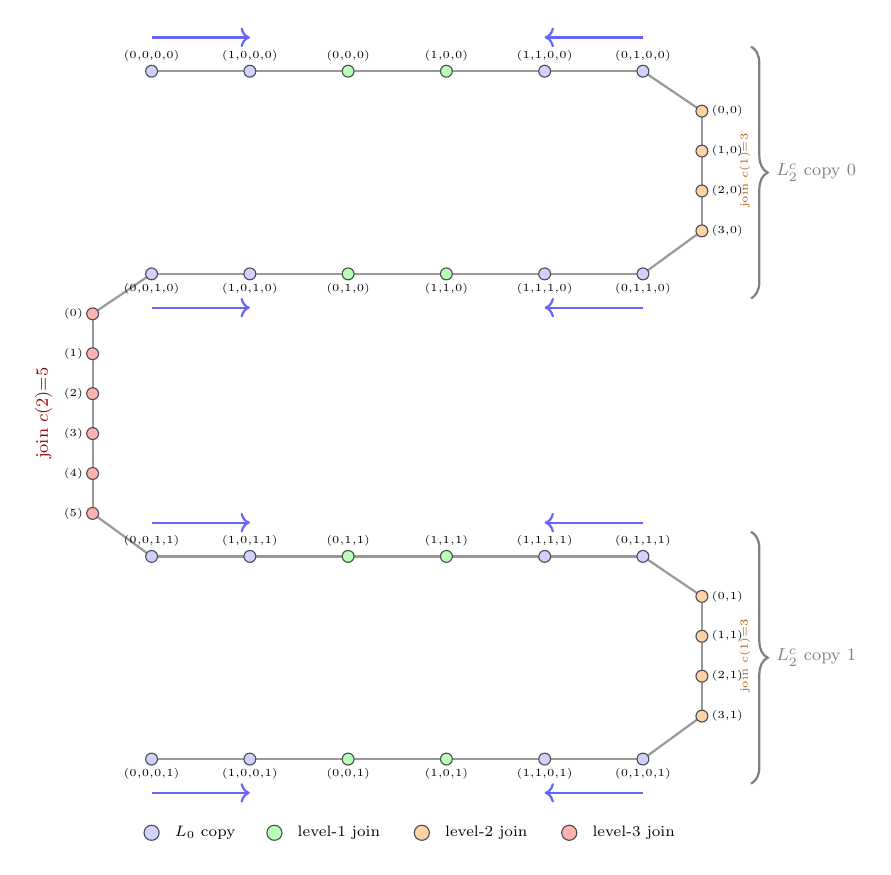
\begin{tikzpicture}[
    scale=0.78, transform shape,
    copycolor/.style={fill=blue!18, draw=black!70},
    joinone/.style={fill=green!28, draw=black!70},
    jointwo/.style={fill=orange!35, draw=black!70},
    jointhree/.style={fill=red!30, draw=black!70},
    nd/.style={circle, minimum size=5.5pt, inner sep=0pt, font=\scriptsize},
    every edge/.style={draw=black!50, thick},
]

% Edges
    \draw[thick, black!40] (0.00,0.00) -- (1.60,0.00);
    \draw[thick, black!40] (1.60,0.00) -- (3.20,0.00);
    \draw[thick, black!40] (3.20,0.00) -- (4.80,0.00);
    \draw[thick, black!40] (4.80,0.00) -- (6.40,0.00);
    \draw[thick, black!40] (6.40,0.00) -- (8.00,0.00);
    \draw[thick, black!40] (8.00,0.00) -- (8.96,-0.65);
    \draw[thick, black!40] (8.96,-0.65) -- (8.96,-1.30);
    \draw[thick, black!40] (8.96,-1.30) -- (8.96,-1.95);
    \draw[thick, black!40] (8.96,-1.95) -- (8.96,-2.60);
    \draw[thick, black!40] (8.96,-2.60) -- (8.00,-3.30);
    \draw[thick, black!40] (8.00,-3.30) -- (6.40,-3.30);
    \draw[thick, black!40] (6.40,-3.30) -- (4.80,-3.30);
    \draw[thick, black!40] (4.80,-3.30) -- (3.20,-3.30);
    \draw[thick, black!40] (3.20,-3.30) -- (1.60,-3.30);
    \draw[thick, black!40] (1.60,-3.30) -- (0.00,-3.30);
    \draw[thick, black!40] (0.00,-3.30) -- (-0.96,-3.95);
    \draw[thick, black!40] (-0.96,-3.95) -- (-0.96,-4.60);
    \draw[thick, black!40] (-0.96,-4.60) -- (-0.96,-5.25);
    \draw[thick, black!40] (-0.96,-5.25) -- (-0.96,-5.90);
    \draw[thick, black!40] (-0.96,-5.90) -- (-0.96,-6.55);
    \draw[thick, black!40] (-0.96,-6.55) -- (-0.96,-7.20);
    \draw[thick, black!40] (-0.96,-7.20) -- (0.00,-7.90);
    \draw[thick, black!40] (0.00,-7.90) -- (1.60,-7.90);
    \draw[thick, black!40] (1.60,-7.90) -- (3.20,-7.90);
    \draw[thick, black!40] (3.20,-7.90) -- (4.80,-7.90);
    \draw[thick, black!40] (4.80,-7.90) -- (6.40,-7.90);
    \draw[thick, black!40] (6.40,-7.90) -- (8.00,-7.90);
    \draw[thick, black!40] (8.00,-7.90) -- (8.96,-8.55);
    \draw[thick, black!40] (8.96,-8.55) -- (8.96,-9.20);
    \draw[thick, black!40] (8.96,-9.20) -- (8.96,-9.85);
    \draw[thick, black!40] (8.96,-9.85) -- (8.96,-10.50);
    \draw[thick, black!40] (8.96,-10.50) -- (8.00,-11.20);
    \draw[thick, black!40] (8.00,-11.20) -- (6.40,-11.20);
    \draw[thick, black!40] (6.40,-11.20) -- (4.80,-11.20);
    \draw[thick, black!40] (4.80,-11.20) -- (3.20,-11.20);
    \draw[thick, black!40] (3.20,-11.20) -- (1.60,-11.20);
    \draw[thick, black!40] (1.60,-11.20) -- (0.00,-11.20);

% Nodes
    \node[nd, copycolor] (v0) at (0.00,0.00) {};
    \node[above=1pt, font=\tiny] at (v0) {$(0{,}0{,}0{,}0)$};
    \node[nd, copycolor] (v1) at (1.60,0.00) {};
    \node[above=1pt, font=\tiny] at (v1) {$(1{,}0{,}0{,}0)$};
    \node[nd, joinone] (v2) at (3.20,0.00) {};
    \node[above=1pt, font=\tiny] at (v2) {$(0{,}0{,}0)$};
    \node[nd, joinone] (v3) at (4.80,0.00) {};
    \node[above=1pt, font=\tiny] at (v3) {$(1{,}0{,}0)$};
    \node[nd, copycolor] (v4) at (6.40,0.00) {};
    \node[above=1pt, font=\tiny] at (v4) {$(1{,}1{,}0{,}0)$};
    \node[nd, copycolor] (v5) at (8.00,0.00) {};
    \node[above=1pt, font=\tiny] at (v5) {$(0{,}1{,}0{,}0)$};
    \node[nd, jointwo] (v6) at (8.96,-0.65) {};
    \node[right=1pt, font=\tiny] at (v6) {$(0{,}0)$};
    \node[nd, jointwo] (v7) at (8.96,-1.30) {};
    \node[right=1pt, font=\tiny] at (v7) {$(1{,}0)$};
    \node[nd, jointwo] (v8) at (8.96,-1.95) {};
    \node[right=1pt, font=\tiny] at (v8) {$(2{,}0)$};
    \node[nd, jointwo] (v9) at (8.96,-2.60) {};
    \node[right=1pt, font=\tiny] at (v9) {$(3{,}0)$};
    \node[nd, copycolor] (v10) at (8.00,-3.30) {};
    \node[below=1pt, font=\tiny] at (v10) {$(0{,}1{,}1{,}0)$};
    \node[nd, copycolor] (v11) at (6.40,-3.30) {};
    \node[below=1pt, font=\tiny] at (v11) {$(1{,}1{,}1{,}0)$};
    \node[nd, joinone] (v12) at (4.80,-3.30) {};
    \node[below=1pt, font=\tiny] at (v12) {$(1{,}1{,}0)$};
    \node[nd, joinone] (v13) at (3.20,-3.30) {};
    \node[below=1pt, font=\tiny] at (v13) {$(0{,}1{,}0)$};
    \node[nd, copycolor] (v14) at (1.60,-3.30) {};
    \node[below=1pt, font=\tiny] at (v14) {$(1{,}0{,}1{,}0)$};
    \node[nd, copycolor] (v15) at (0.00,-3.30) {};
    \node[below=1pt, font=\tiny] at (v15) {$(0{,}0{,}1{,}0)$};
    \node[nd, jointhree] (v16) at (-0.96,-3.95) {};
    \node[left=1pt, font=\tiny] at (v16) {$(0)$};
    \node[nd, jointhree] (v17) at (-0.96,-4.60) {};
    \node[left=1pt, font=\tiny] at (v17) {$(1)$};
    \node[nd, jointhree] (v18) at (-0.96,-5.25) {};
    \node[left=1pt, font=\tiny] at (v18) {$(2)$};
    \node[nd, jointhree] (v19) at (-0.96,-5.90) {};
    \node[left=1pt, font=\tiny] at (v19) {$(3)$};
    \node[nd, jointhree] (v20) at (-0.96,-6.55) {};
    \node[left=1pt, font=\tiny] at (v20) {$(4)$};
    \node[nd, jointhree] (v21) at (-0.96,-7.20) {};
    \node[left=1pt, font=\tiny] at (v21) {$(5)$};
    \node[nd, copycolor] (v22) at (0.00,-7.90) {};
    \node[above=1pt, font=\tiny] at (v22) {$(0{,}0{,}1{,}1)$};
    \node[nd, copycolor] (v23) at (1.60,-7.90) {};
    \node[above=1pt, font=\tiny] at (v23) {$(1{,}0{,}1{,}1)$};
    \node[nd, joinone] (v24) at (3.20,-7.90) {};
    \node[above=1pt, font=\tiny] at (v24) {$(0{,}1{,}1)$};
    \node[nd, joinone] (v25) at (4.80,-7.90) {};
    \node[above=1pt, font=\tiny] at (v25) {$(1{,}1{,}1)$};
    \node[nd, copycolor] (v26) at (6.40,-7.90) {};
    \node[above=1pt, font=\tiny] at (v26) {$(1{,}1{,}1{,}1)$};
    \node[nd, copycolor] (v27) at (8.00,-7.90) {};
    \node[above=1pt, font=\tiny] at (v27) {$(0{,}1{,}1{,}1)$};
    \node[nd, jointwo] (v28) at (8.96,-8.55) {};
    \node[right=1pt, font=\tiny] at (v28) {$(0{,}1)$};
    \node[nd, jointwo] (v29) at (8.96,-9.20) {};
    \node[right=1pt, font=\tiny] at (v29) {$(1{,}1)$};
    \node[nd, jointwo] (v30) at (8.96,-9.85) {};
    \node[right=1pt, font=\tiny] at (v30) {$(2{,}1)$};
    \node[nd, jointwo] (v31) at (8.96,-10.50) {};
    \node[right=1pt, font=\tiny] at (v31) {$(3{,}1)$};
    \node[nd, copycolor] (v32) at (8.00,-11.20) {};
    \node[below=1pt, font=\tiny] at (v32) {$(0{,}1{,}0{,}1)$};
    \node[nd, copycolor] (v33) at (6.40,-11.20) {};
    \node[below=1pt, font=\tiny] at (v33) {$(1{,}1{,}0{,}1)$};
    \node[nd, joinone] (v34) at (4.80,-11.20) {};
    \node[below=1pt, font=\tiny] at (v34) {$(1{,}0{,}1)$};
    \node[nd, joinone] (v35) at (3.20,-11.20) {};
    \node[below=1pt, font=\tiny] at (v35) {$(0{,}0{,}1)$};
    \node[nd, copycolor] (v36) at (1.60,-11.20) {};
    \node[below=1pt, font=\tiny] at (v36) {$(1{,}0{,}0{,}1)$};
    \node[nd, copycolor] (v37) at (0.00,-11.20) {};
    \node[below=1pt, font=\tiny] at (v37) {$(0{,}0{,}0{,}1)$};

% Direction arrows for L_0 copies
    \draw[->, thick, blue!60] (0.00,0.55) -- (1.60,0.55);
    \draw[->, thick, blue!60] (8.00,0.55) -- (6.40,0.55);
    \draw[->, thick, blue!60] (8.00,-3.85) -- (6.40,-3.85);
    \draw[->, thick, blue!60] (0.00,-3.85) -- (1.60,-3.85);
    \draw[->, thick, blue!60] (0.00,-7.35) -- (1.60,-7.35);
    \draw[->, thick, blue!60] (8.00,-7.35) -- (6.40,-7.35);
    \draw[->, thick, blue!60] (8.00,-11.75) -- (6.40,-11.75);
    \draw[->, thick, blue!60] (0.00,-11.75) -- (1.60,-11.75);

% Structural braces
    \draw[decorate, decoration={brace, amplitude=6pt}, thick, black!50]
        (9.76,0.40) -- (9.76,-3.70)
        node[midway, right=8pt, font=\footnotesize] {$L^c_2$ copy $0$};
    \draw[decorate, decoration={brace, amplitude=6pt}, thick, black!50]
        (9.76,-7.50) -- (9.76,-11.60)
        node[midway, right=8pt, font=\footnotesize] {$L^c_2$ copy $1$};
    \node[font=\footnotesize, text=red!60!black] at (-1.76,-5.57) {\rotatebox{90}{join $c(2){=}5$}};
    \node[font=\tiny, text=orange!70!black] at (9.66,-1.62) {\rotatebox{90}{join $c(1){=}3$}};
    \node[font=\tiny, text=orange!70!black] at (9.66,-9.52) {\rotatebox{90}{join $c(1){=}3$}};

% Legend
    \node[nd, copycolor, minimum size=7pt] at (0,-12.40) {};
    \node[right=3pt, font=\scriptsize] at (0.15,-12.40) {$L_0$ copy};
    \node[nd, joinone, minimum size=7pt] at (2.0,-12.40) {};
    \node[right=3pt, font=\scriptsize] at (2.15,-12.40) {level-1 join};
    \node[nd, jointwo, minimum size=7pt] at (4.4,-12.40) {};
    \node[right=3pt, font=\scriptsize] at (4.55,-12.40) {level-2 join};
    \node[nd, jointhree, minimum size=7pt] at (6.8,-12.40) {};
    \node[right=3pt, font=\scriptsize] at (6.95,-12.40) {level-3 join};
\end{tikzpicture}}
    \end{column}
  \end{columns}
\end{frame}

% ============================================================
% SECTION 2b — Deep Computations: a glimpse (Chapter 3)
% Brief, informal main-flow addition per Tona's request: quick CCS
% reminder, the general worry that closures can be "wild" (non-Baire-1),
% the BFT dichotomy as the tool that rules this out, and two concrete
% examples (Cantor threshold classifiers, prefix/equality tests) whose
% closures turn out to be tame. Source: chapters/3-deep-computations/
% 01-intro.tex and 03-examples-CCS.tex, Subsec. sec:Cantor-classifiers
% and sec:prefix-test.
% ============================================================
\section{Deep Computations: a Glimpse}

\begin{frame}{Why closures can misbehave}
  A \textbf{CCS} $(L,\mathcal P,\Gamma)$ has states $L$, observable predicates $\mathcal P$, and a monoid $\Gamma\subseteq L^L$ of computations; \textbf{deep computations} are the closure $\overline\Gamma$.
  \vspace{0.3em}

  The worry: closures of families of continuous functions need \alert{not} stay ``nice''.
  \vspace{0.3em}

  \begin{block}{The BFT dichotomy (Bourgain--Fremlin--Talagrand) fixes this}
    For bounded $A\subseteq \Cp(X)$, $A$'s closure consists entirely of \alert{Baire-1 functions} $\iff$ $A$ has \textbf{NIP} (non-independence property).
  \end{block}
  NIP is exactly the dividing line between ``the closure stays tame'' and ``the closure can go wild.''
\end{frame}

\begin{frame}{The Todor\v{c}evi\'c trichotomy}
  \begin{block}{Theorem (Todor\v{c}evi\'c, 1999)}
    Let $K$ be a separable Rosenthal compactum: either $K$ is metrizable, or one of three ``minimal'' non-metrizable compacta embeds into $K$.
  \end{block}
  \centering
  \resizebox{!}{3.8cm}{%figures/separable-compacta.tex

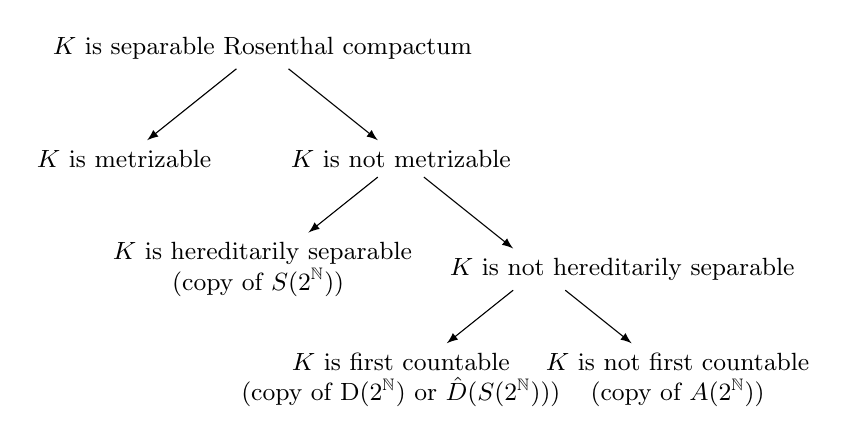
\begin{tikzpicture}[grow=down,
    sibling distance=10em,
    level distance=4em,
    edge from parent/.style={draw,-latex},
    every node/.style={font=\small,align=center}]

\node {$K$ is separable Rosenthal compactum}
    child {node {$K$ is metrizable}}
    child {node {$K$ is not metrizable}
    child {node {$K$ is hereditarily separable \\ (copy of $S(2^\mathbb{N})$) \hspace{2cm}}}
    child {node {\hspace{2cm} $K$ is not hereditarily separable}
    child {node {$K$ is first countable \\ (copy of $\mathrm{D}(2^\mathbb{N})$ or $\hat{D}(S(2^\mathbb{N}))$)}}
    child {node {$K$ is not first countable \\ (copy of $A(2^\mathbb{N})$)}}}};
\end{tikzpicture}}

  Our two examples (next slide) sit at opposite corners of this trichotomy.
\end{frame}

\begin{frame}{Two examples: tame closures on Cantor space}
  \begin{block}{Threshold classifiers}
    $x\preccurlyeq_n w$: is $x\restriction_n \preceq w$? Continuous, definable. \textbf{Closure} = ``ultra-classifiers'' $\preceq z,\ \prec z$ ($z\in 2^{\mathbb N}$): a \emph{split Cantor set} $\cong 2^{\mathbb N}\times\{0,1\}$, \alert{hereditarily separable, non-metrizable}.
  \end{block}
  \begin{block}{Prefix tests}
    $x\equiv_n w$: is $w$ the length-$n$ prefix of $x$? Continuous, definable. \textbf{Closure} = $\mathbf 0$, finite-prefix tests, or point-\emph{equality} tests $\bar x: y\mapsto\Brack{y=x}$, separable, but \alert{not first countable}.
  \end{block}
  Takeaway: ``tame'' doesn't mean ``simple,'' just that every limit is describable.
\end{frame}

\begin{frame}{The chapter's main theorem: BFT for CCS}
  Combined with the Todor\v{c}evi\'c trichotomy, this yields a hierarchy of \alert{four} tameness classes, $\mathrm{NIP}_3\Rightarrow\mathrm{NIP}_2\Rightarrow\mathrm{NIP}_1\Rightarrow\mathrm{NIP}$.

  Our two examples above witness two of these separations; the thesis exhibits examples separating every level.
\end{frame}

% ============================================================
% SECTION 3 — Amoeba Graphs and the Feasible Edge-Replacement Group
% (combinatorics — lighter weight but real depth: ~12-15 min,
% ~7-9 frames). Molloy is likely to engage here — don't shortchange.
% Likely source: Chapter 4 files (intro, border tracing, recursive
% constructions, amoeba trees, infinitary amoebas)
% ============================================================
\section{The Group of Feasible Edge Replacements}

\begin{frame}{The \tFer Group (Caro--Hansberg--Montejano)}
  \begin{center}
  \textbf{$C_4$ is rigid}: two isomorphic labelled 4-cycles, connected by \emph{no} sequence of feasible edge replacements.
  \end{center}
  \begin{figure}
  \centering
  % figures/4-cycles.tex

% Left Subfigure: "U-shape" path
\begin{subfigure}[b]{0.4\textwidth}
    \centering
    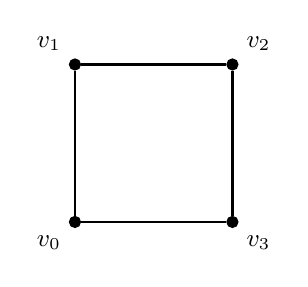
\begin{tikzpicture}[scale=2]
        % Define coordinates for a square
        \node[vertex, label={[vlabel]above left:$v_1$}] (TL) at (0,1) {};
        \node[vertex, label={[vlabel]above right:$v_2$}] (TR) at (1,1) {};
        \node[vertex, label={[vlabel]below left:$v_0$}] (BL) at (0,0) {};
        \node[vertex, label={[vlabel]below right:$v_3$}] (BR) at (1,0) {};

        % Draw the path: Left, Top, Right
        \draw[thick] (BL) -- (TL) -- (TR) -- (BR) -- (BL);
    \end{tikzpicture}
\end{subfigure}
\hfill
% Right Subfigure: "Z-shape" / Diagonals
\begin{subfigure}[b]{0.4\textwidth}
    \centering
    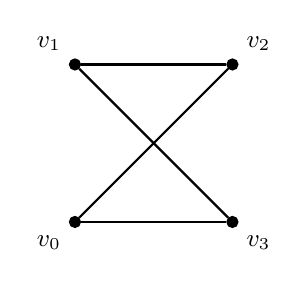
\begin{tikzpicture}[scale=2]
        % Define coordinates for a square
        \node[vertex, label={[vlabel]above left:$v_1$}] (TL) at (0,1) {};
        \node[vertex, label={[vlabel]above right:$v_2$}] (TR) at (1,1) {};
        \node[vertex, label={[vlabel]below left:$v_0$}] (BL) at (0,0) {};
        \node[vertex, label={[vlabel]below right:$v_3$}] (BR) at (1,0) {};

        % Draw the path: Bottom-Left to Top-Left, Top-Left to Bottom-Right, Bottom-Right to Top-Right
        % Based on your description: "top edge and the two diagonals"
        \draw[thick] (BL) -- (TR); % Diagonal 1
        \draw[thick] (TR) -- (TL); % Top edge
        \draw[thick] (TL) -- (BR); % Diagonal 2
        \draw[thick] (BL) -- (BR);
    \end{tikzpicture}
\end{subfigure}

  \end{figure}
  \vspace{0.6em}
  \begin{center}
  \textbf{The puzzle}: two isomorphic labelled copies of $P_4$. Can one reach the other?
  \end{center}
  \begin{figure}
  \centering
  \input{../figures/4-paths.tex}
  \end{figure}
\end{frame}

\begin{frame}{A twist at infinity: the bi-infinite path $P_{\mathbb Z}$}
  \begin{figure}
  \centering
  \resizebox{0.68\textwidth}{!}{% figures/infinite-paths.tex

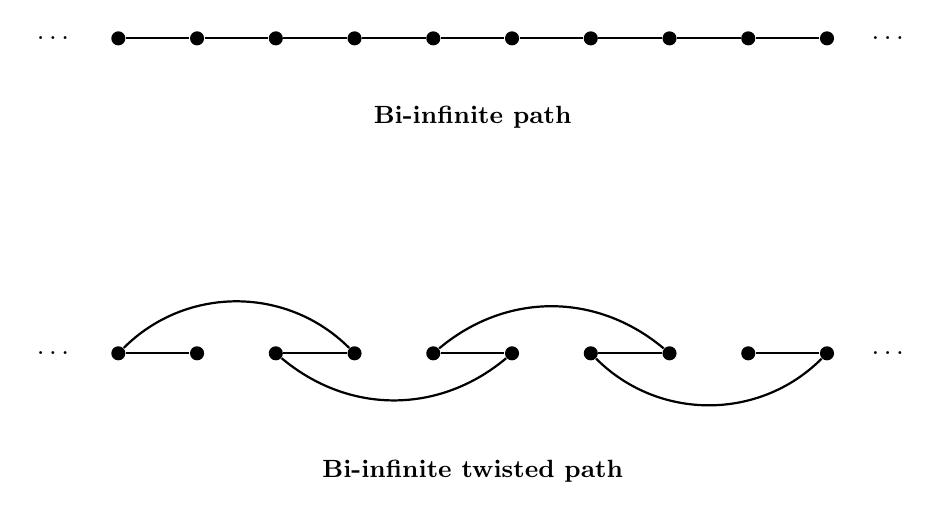
\begin{tikzpicture}[
    vertex/.style={circle, fill, inner sep=1.8pt},
    edge/.style={thick},
    caption/.style={font=\small\bfseries, node distance=1.5cm}
]

    % --- Subfigure 1: Bi-infinite Path (Top) ---
    \begin{scope}[yshift=4cm]
        % Vertices -4 to 5
        \foreach \x in {-4,...,5}
            \node[vertex] (v\x) at (\x, 0) {};
            
        % Consecutive horizontal edges
        \foreach \x [evaluate=\x as \nextx using int(\x+1)] in {-4,...,4}
            \draw[edge] (v\x) -- (v\nextx);
            
        % Continuation dots
        \node at (-4.8, 0) {$\dots$};
        \node at (5.8, 0) {$\dots$};
        
        % Caption for the first graph
        \node[caption] at (0.5, -1) {Bi-infinite path};
    \end{scope}

    % --- Subfigure 2: Matching and Arcs (Bottom) ---
    \begin{scope}[yshift=0cm]
        % Vertices -4 to 5
        \foreach \x in {-4,...,5}
            \node[vertex] (u\x) at (\x, 0) {};
            
        % Specified horizontal edges (the matching)
        \foreach \a/\b in {-4/-3, -2/-1, 0/1, 2/3, 4/5}
            \draw[edge] (u\a) -- (u\b);
            
        % Upper arcs
        \draw[edge] (u-4) to[bend left=45] (u-1);
        \draw[edge] (u0) to[bend left=40] (u3);
        
        % Lower arcs
        \draw[edge] (u-2) to[bend right=40] (u1);
        \draw[edge] (u2) to[bend right=45] (u5);

        % Continuation dots
        \node at (-4.8, 0) {$\dots$};
        \node at (5.8, 0) {$\dots$};
        
        % Caption for the second graph
        \node[caption] at (0.5, -1.5) {Bi-infinite twisted path};
    \end{scope}

\end{tikzpicture}}
  \end{figure}

  This entire infinitary strand is \alert{sole-authored}.
\end{frame}

\begin{frame}{Main results}
  \begin{block}{Fibonacci-type trees $T_k$ (with Eslava et al.)}
    $T_k$ is a local amoeba for every $k$, with matching extremal bounds on how unbalanced a 2-colouring of $K_n$ can be forced to stay.
  \end{block}
  \begin{figure}
  \centering
  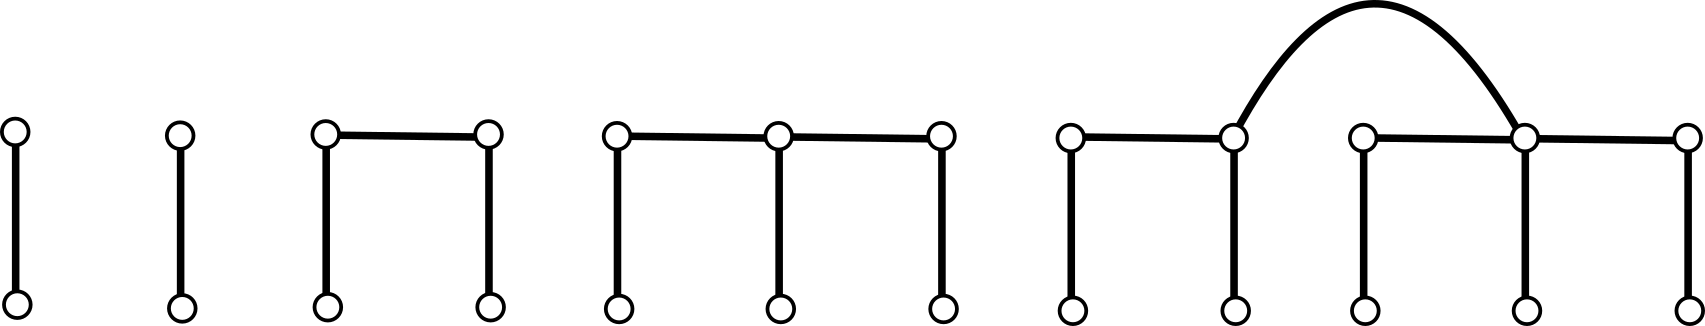
\includegraphics[scale=0.2]{../images/fibonacci_trees.png}
  \end{figure}
\end{frame}

\begin{frame}{Zooming out: the rest of the chapter}
  $T_k$ is one instance of a broader programme. The chapter also:
  \begin{itemize}
    \item builds \textbf{other families} of trees with large $\Fer$ groups, each paired with extremal (Tur\'an-type) bounds;
    \item gives a \textbf{structural classification} for finite trees: exactly when $\Aut(T)$ already equals $\Fer(T)$ (rigidity) versus when it is much larger;
    \item extends everything to \textbf{countably infinite} graphs, where $\Fer(G)$ is a Polish group, classifying rigidity via the ends of the tree;
    \item takes the first steps toward a \textbf{descriptive-set-theoretic} version of the same questions, for analytic (not just countable) graphs.
  \end{itemize}
\end{frame}

\begin{frame}{The infinitary case: Baire-category \texorpdfstring{$\bal=\ex$}{bal=ex}}
  Extending to $X$ countably infinite: $S_X$ becomes a Polish group, $\Fer(G)$ an analytic subgroup.
  \begin{block}{Theorem (infinitary analogue of the Eslava et al.\ identity)}
    Let $X$ be a perfect Polish space, $G$ a finite global amoeba, and $c\colon[X]^2\to 2$ a Baire-measurable colouring with non-meagre colour classes. Then there is a \emph{balanced} copy of $G$.
  \end{block}
\end{frame}

% ============================================================
% CONCLUSION
% ============================================================
\section{Conclusion}

\begin{frame}{Summary}
  \begin{quote}
    ``This thesis studies the cost of insisting on definable solutions.''
  \end{quote}
  \begin{itemize}
    \item \textbf{Dichromatic number}: the basis paradigm for finite thresholds is now fully settled, undirected \emph{and} directed. The last piece was $\mathbf\Sigma^1_2$-completeness of Borel 2-dicolouring.
    \item \textbf{Deep computations}: a four-level NIP hierarchy for when limits of computations stay tame, with two new separating examples.
    \item \textbf{\tFer group}: a Polish group action encoding a combinatorial notion of rigidity, now with an infinitary Baire-categorical extension.
  \end{itemize}
\end{frame}

\begin{frame}{Open problems}
  \begin{itemize}
    \item \textbf{Dichromatic number}: does every basis for $\vec\chi_B(D)>\aleph_0$ (Raghavan--Xiao) have size $\mathfrak c$, or is there a smaller one? Does a countable basis exist for structurally simpler classes (e.g.\ directed graphs generated by a single Borel function)?
    \textbf{My conjecture:} there is no countable basis. Preparing draft for submission.
    \item \textbf{\tFer group (infinitary)}: characterize the countably infinite, locally finite trees that are local amoebas. Is $\overline{\Fer(T)}$ always amenable for non-rigid trees? Is the local-amoeba property itself Borel?
  \end{itemize}
\end{frame}

\begin{frame}
  \centering
  {\Large Thank you}

  \vspace{1em}
  \normalsize Questions?
\end{frame}

% ============================================================
% BACKUP SLIDES — not part of the main talk; pulled up only if the
% relevant question comes up.
%
% To compile a version WITHOUT this section (e.g. to send someone a
% preview that ends at "Thank you"), compile slides-advisor.tex instead
% of this file — it just \defs \NoBackupSlides then \inputs this file,
% which skips everything between here and \end{document}.
% ============================================================
\ifdefined\NoBackupSlides
\else
\appendix
\section{Backup}

\begin{frame}{Backup: dichromatic number setup}
  \begin{itemize}
    \item $G$ ranges over \alert{analytic graphs}: $V(G)=X$ Polish, edge relation analytic in $X\times X$.
    \item $\chi_B(G)$: least $k$ such that $G$ admits a Borel proper $k$-colouring.
    \item A \alert{directed graph} $D$ has arcs (ordered pairs). A \alert{dicolouring} $c\colon V(D)\to k$ requires each colour class to induce an \emph{acyclic} subgraph.
    \item $\vec\chi(D)$ / $\vec\chi_B(D)$: least $k$ for a (Borel) dicolouring.
    \item Borel graphs/digraphs are studied via \alert{nice codes} (Thornton): reals coding Borel sets, compatible with $\Sigma^1_1$/$\Pi^1_1$ definitions of the coded set. ``$\mathbf\Sigma^1_2$-complete'' is a statement about the complexity of the set of codes.
  \end{itemize}
\end{frame}

\begin{frame}{Backup: dichromatic number, minimal monochromatic cycles}
  Why does a 2-dicolouring of $H$'s gadget copies glue to a 2-dicolouring of $D(H)$? The naive hope ``each gadget is locally fine, so the whole graph is fine'' needs repair, since a monochromatic cycle need \alert{not} stay inside one gadget copy.
  \begin{enumerate}
    \item Take a monochromatic directed cycle $C$ of \emph{minimal length} (for contradiction).
    \item Arcs between original hypergraph vertices respect a fixed linear order $\Rightarrow$ $C$ cannot lie entirely in $V$.
    \item $C$ cannot lie entirely in one gadget $F_e$ either (each $\sigma(e)$ is a genuine 2-dicolouring of $F_e$).
    \item So $C$ crosses a gadget via a segment $x\to\cdots\to y\to\cdots\to z$, $y$ auxiliary, $x,z\in\{a,b,c\}$.
    \item Minimality $\Rightarrow$ no shortcut arc $x\to z$ $\Rightarrow$ $(x,z)\notin E(F)$ $\Rightarrow$ (checking $F$'s three shared-to-shared arcs $a\to b, a\to c, b\to c$) forces the arc $z\to x$.
    \item But then $z\to x$ plus the segment $x\to\cdots\to z$ is a \emph{monochromatic cycle entirely inside $F_e$}: a contradiction.
  \end{enumerate}
\end{frame}

\begin{frame}{Backup: $\mathbb L_0$, two ways to prove a perfect set theorem}
  Both strategies analyze the pruned tree $T\subseteq 2^{<\omega}$ with $C=[T]$:
  \begin{itemize}
    \item \textbf{Iterative derivation}: iteratively delete nodes with $\leq 1$ branch above them, through the countable ordinals. (Original KST proof of the $\mathbb G_0$ dichotomy.)
    \item \textbf{Condensation}: keep only nodes above which $C$ is uncountable, in \emph{one step}. (Bernshteyn's newer proof of $\mathbb G_0$.)
  \end{itemize}
  Equivalent in strength for $2^{<\omega}$, but condensation is more economical and, unlike iterative derivation, needs a form of choice that fails under $\mathsf{AD}$.
\end{frame}

\begin{frame}{Backup: $\mathbb L_0$ setup}
  \begin{itemize}
    \item Fix $c\in\omega^\omega$. Build finite paths $L^c_n$ recursively: $L^c_{n+1}$ joins \emph{two copies} of $L^c_n$ by a fresh path of $c(n)+2$ edges.
    \item $\mathbb L_c$ is the natural limit graph: vertices are $(m,k,x)$ with $x\in 2^\omega$ recording, at each stage, which of the two copies a point falls in.
    \item If $c$ is unbounded and odd-valued: $\mathbb L_c$ is an acyclic graph of degree $\leq 2$, and $\chi_B(\mathbb L_c)=3$.
    \item Fixing one canonical such $c_0$: $\mathbb L_0 := \mathbb L_{c_0}$.
  \end{itemize}
\end{frame}

\begin{frame}{Backup: $\mathbb L_0$ main theorem}
  The dichotomy follows from combining two theorems:
  \begin{block}{Theorem A}
    For any analytic graph $G$: either $\chi_B(G)\leq 2$, or $\mathbb L_c\to_c G$ for some unbounded, odd-valued $c$.
  \end{block}
  \begin{block}{Theorem B}
    For $c,d$ unbounded and odd-valued, $\mathbb L_c$ and $\mathbb L_d$ are continuously homomorphically equivalent.
  \end{block}
  Theorem B is purely combinatorial and does not depend on how Theorem A is proved.
\end{frame}

\begin{frame}{Backup: $\mathbb L_0$ proof strategy: condensation}
  Central device: a $\sigma$-ideal of \alert{small} sets of homomorphisms $\mathcal L\subseteq\Hom(L^c_n,G)$.
  \begin{itemize}
    \item $\Phi(A,k)$: $A$ is analytic and all odd walks of $G$ with endpoints in $A$ have length $\leq 2k-1$.
    \item $\mathcal L$ is \emph{tiny} if $\Phi(\mathcal L(u),k)$ for some vertex $u$ and some $k$; \emph{small} = countable union of tiny sets; \emph{large} = not small.
    \item Key fact: if $\Phi(A,n)$, then $A$'s connected component is contained in an invariant Borel 2-colourable set (via analytic $\Rightarrow$ Borel separation).
  \end{itemize}
  So: $\chi_B(G)>2 \Rightarrow X$ itself is large (as $\Hom(\bullet,G)$). Recursively build a nested sequence of \emph{large} Borel sets $\mathcal L_n\subseteq\Hom(L^c_n,G)$ of shrinking diameter, dynamically choosing $c(n)$ at each stage; a continuous homomorphism $\mathbb L_c\to G$ falls out as the Cantor-intersection limit.
\end{frame}

\begin{frame}{Backup: $\mathbb L_0$ key lemma: largeness survives doubling}
  The crux is showing largeness can always be preserved when doubling $L^c_n\to L^c_{n+1}$:
  \begin{block}{Lemma}
    If $\mathcal L\subseteq\Hom(L^c_n,G)$ is large, then for any $N$ there is an odd $d(n)\geq N$ such that $\mathcal L^{+d}$ (the set of homomorphisms restricting to $\mathcal L$ on both new copies) is again large.
  \end{block}
  \textbf{Why}: suppose not, then every choice of gap length decomposes $\mathcal L^{+d}$ into countably many tiny pieces. Each tiny witness (an analytic set with a $\Phi$-bound) can be reflected up to a \alert{Borel} set with the same bound, via the \textbf{First Reflection Theorem} ($\Pi^1_1$-on-$\Sigma^1_1$). Removing all these countably many Borel-tiny pieces from $\mathcal L$ leaves a large remainder, which produces a genuine counterexample, a contradiction.
\end{frame}

\begin{frame}{Backup: contribution \S2.4 Cantor game}
  % Leave room to fold in coauthor comments if Spencer forwards any before the defence.
  \textbf{MW, Salvetti} (\emph{Uncountable sets and an infinite linear order game}, Topology Proceedings 2025).
  \vspace{0.5em}

  My contribution: equal contribution throughout the results, the writing, and the submission.
\end{frame}

\begin{frame}{Backup: contribution \S3 Deep Computations}
  \textbf{Due\~nez, Iovino, MW, Salvetti, Tall} (\emph{Complexity of Deep Computations via Topology of Function Spaces}, arXiv 2026).
  \vspace{0.5em}

  My contribution: constructed the two examples used to separate the $\mathrm{NIP}_i$ hierarchy, threshold classifiers on Cantor space (witnessing $\mathrm{NIP}_2\not\Rightarrow\mathrm{NIP}_3$) and prefix/equality tests (witnessing $\mathrm{NIP}\not\Rightarrow\mathrm{NIP}_1$). Presented this material extensively at the Fields Institute seminar series (2024--2026) and contributed substantially to drafting and revising the paper.
\end{frame}

\begin{frame}{Backup: contribution \S4.2 Border tracing}
  \textbf{P.~Wiederhold, MW} (\emph{Border tracing in oriented adjacency graphs...}, TCS 2026).
  \vspace{0.5em}

  My contribution: co-developed the border-tracing algorithms, including the corrected End Condition Test, and their edge-case analysis; independently designed, implemented, and documented an object-oriented framework realizing the algorithms, with a test suite validating contour detection on square, triangular, and hexagonal tilings.
\end{frame}

\begin{frame}{Backup: contribution \S4.3 Recursive constructions}
  \textbf{Eslava, Hansberg, MW, Ventura} (\emph{New recursive constructions of amoebas...}, Aequationes Math.\ 2025) Fibonacci-type trees $T_k$, balancing number bounds.
  \vspace{0.5em}

  My contribution: substantial, co-equal contribution to the main result that the trees are local amoebas; equal contribution to the remaining joint sections. Independently wrote Section 5 (the recursive algorithm and its complexity analysis) and independently designed and implemented the accompanying object-oriented framework, including the abstract classes for feasible edge replacements.
\end{frame}

\begin{frame}{Backup: contribution \S4.3 Constant balancing number}
  \textbf{Caro, Gonz\'alez, Hansberg, J\'acome, MW, Montejano} (\emph{Graphs with constant balancing number}, Procedia CS 2023).
  \vspace{0.5em}

  My contribution: equal contribution to the paper's main results, the structural characterization of constant-balancing-number graphs.
\end{frame}

\begin{frame}{Backup: contribution \S4.4 Amoeba trees}
  \textbf{G\'omez, Gonz\'alez, Hansberg, MW} (\emph{Amoeba trees}, in preparation) structural theory of $\Fer(T)$ vs.\ $\Aut(T)$.
  \vspace{0.5em}

  My contribution: originated the paper's central conjecture, that the \tFer group of every global amoeba tree has at most two orbits, and extended the object-oriented framework with a statistics database used to find counterexamples and formulate further conjectures; equal contribution to the proofs and main results.
\end{frame}

\begin{frame}{Backup: sole-authored work}
  Sole-authored, under Spencer Unger's supervision:
  \begin{itemize}
    \item \S2.2 the new $\mathbb L_0$ proof;
    \item \S2.3 the $\Sigma^1_2$-completeness / dichromatic number result;
  \end{itemize}
  \vspace{0.5em}
  Sole-authored:
  \begin{itemize}
    \item \S4.5 the infinitary \tFer-group strand.
  \end{itemize}
\end{frame}

\begin{frame}{Backup: \tFer group setup}
  Fix a labelling $\lambda\colon V(G)\to X$. For $e\in E(G)$, $f\in E(G^c)$ non-edge, write $\sigma::(e\to f)$ if the label permutation $\sigma$ induces an isomorphism $\varphi_\sigma\colon G\to G-e+f$.
  \begin{itemize}
    \item $\Fer(G) := \langle\, \sigma : \sigma::(e\to f) \text{ for some } e,f \,\rangle \leq S_X$, the \alert{canonical generators} include $A(G):=\{\sigma:\varphi_\sigma\in\Aut(G)\}$ and all single-edge moves.
    \item $1 \leq A(G) \leq \Fer(G) \leq S_X$.
    \item $G$ is a \textbf{local amoeba} if $\overline{\Fer(G)}=S_X$ (every relabelling is reachable); \textbf{rigid} if $\overline{\Fer(G)}=A(G)$ (no non-automorphism move exists).
    \item $G$ is a \textbf{global amoeba} if $G\cup tK_1$ (add $t$ isolated vertices) is a local amoeba for some $t\geq 1$.
  \end{itemize}
  Example: $\Fer(C_4)=A(C_4)=D_4$ (rigid); $\Fer(P_4)=S_4$ (local amoeba).
\end{frame}

\begin{frame}{Backup: \tFer group infinitary constant balancing}
  Extending to $X$ countably infinite: $S_X$ becomes a Polish group, $\Fer(G)$ an analytic subgroup.
  \begin{block}{Theorem (infinitary analogue of the Caro et al.\ characterization)}
    Let $c\colon[X]^2\to 2$ be a Baire-measurable colouring of a perfect Polish space $X$ with non-meagre colour classes. Then some colour $i$, vertex $v_0$, and Cantor set $C$ satisfy: every edge $v_0$--$C$ has colour $i$, and $[C]^2$ is monochromatic in colour $1-i$ (a continuum-size star \emph{and} a continuum-size clique).
  \end{block}
\end{frame}

\begin{frame}{Backup: \tFer group complexity \& border tracing}
  \begin{itemize}
    \item \textbf{$O(n\log n)$ decomposition.} Factoring an arbitrary permutation of $T_k$ into feasible edge replacements: the published algorithm's analysis gives $\Theta(n^2)$ time (Eslava et al., Thm.~11).
    \item \textbf{Computational framework.} The \tfer object formalism is implemented as an open-source object-oriented framework for experimenting with feasible edge replacements.
    \item \textbf{Border tracing} (peripheral side project): a corrected version of Voss' Border Mesh Determination Algorithm for oriented adjacency graphs of polygonal tilings (square/triangular/hexagonal).
  \end{itemize}
\end{frame}

\begin{frame}{Backup: \tFer group, genuinely rigid graphs}
  Schweitzer--Schweitzer (2017, resolving a Ne\v{s}et\v{r}il conjecture): exactly \alert{18} minimal asymmetric graphs. Does an analogous finite classification hold for $\Fer$-rigidity?
  \begin{itemize}
    \item Naive translation fails: odd cycles $C_{2n+1}$ are rigid \emph{vacuously}.
    \item Fix: $G$ is \textbf{genuinely rigid} if $\Fer(G)=A(G)$ \emph{and} some degree-preserving replacement exists.
    \item Smallest example: $K_{2,3}$.
  \end{itemize}
  \begin{block}{Question}
    Are there finitely many \emph{minimal} genuinely rigid graphs?
  \end{block}
\end{frame}

\begin{frame}{Backup: Newton's method 1}
  \textbf{Newton CCS for $\rho(z)=z^3-2z+2$:} states $L=\hatC$; predicates $\mathcal P=(P_1,P_2,P_3)$ (stereographic coordinates); computations $\Gamma_\rho=\{N_\rho^{(n)}\}$, where $N_\rho(z)=z-\frac{\rho(z)}{\rho'(z)}=\frac{2z^3-2}{3z^2-2}$.

  Colour $z_0$ by the nearest root to $N_\rho^{(n)}(z_0)$.
  \begin{center}
    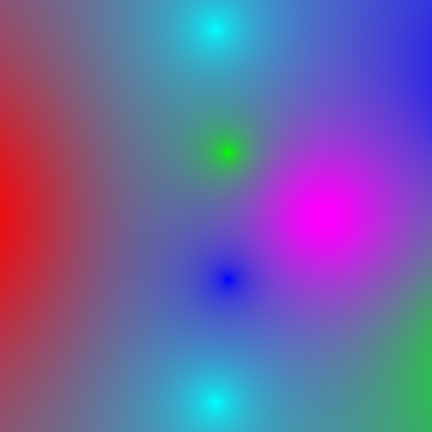
\includegraphics[width=0.24\textwidth]{../images/newton_div1.png}\hfill
    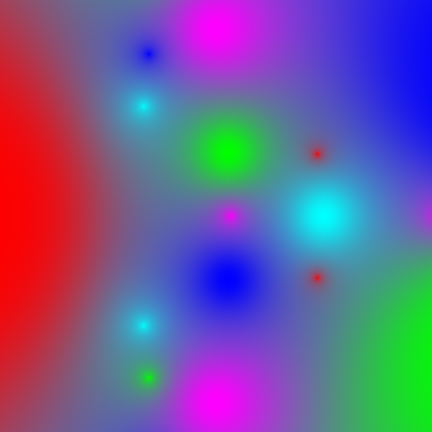
\includegraphics[width=0.24\textwidth]{../images/newton_div2.png}\hfill
    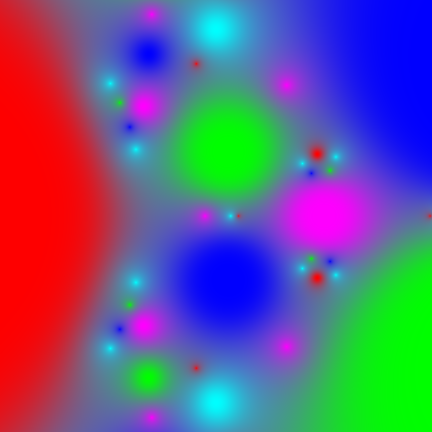
\includegraphics[width=0.24\textwidth]{../images/newton_div3.png}
  \end{center}
\end{frame}

\begin{frame}{Backup: Newton's method 2}
  On most of $\hatC$, the \textbf{deep computation} \emph{is} a root of $\rho$.

  But from $z_0=0$: $N_\rho^{(\bullet)}(0) = (0,1,0,1,\dots)$ \alert{never converges}, yet its even and odd subsequences do, to two \emph{different} deep computations $f_0\equiv 0$ and $f_1\equiv 1$; neither is a root.
  \begin{center}
    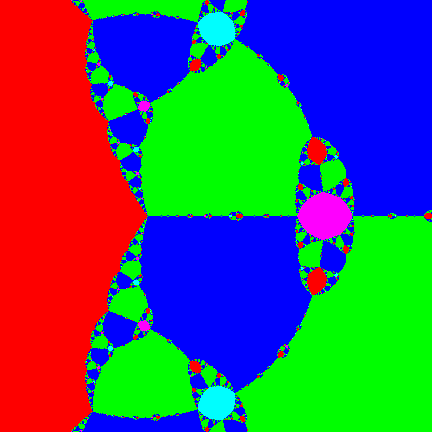
\includegraphics[width=0.23\textwidth]{../images/newton_div99.png}\hfill
    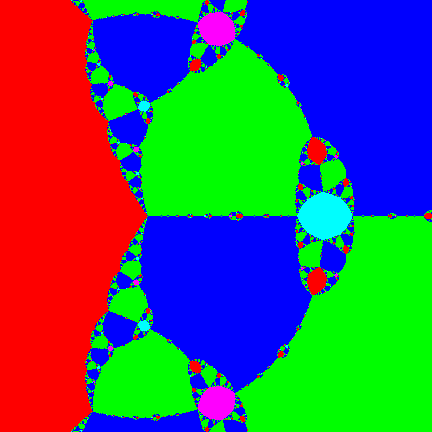
\includegraphics[width=0.23\textwidth]{../images/newton_div100.png}\hfill
    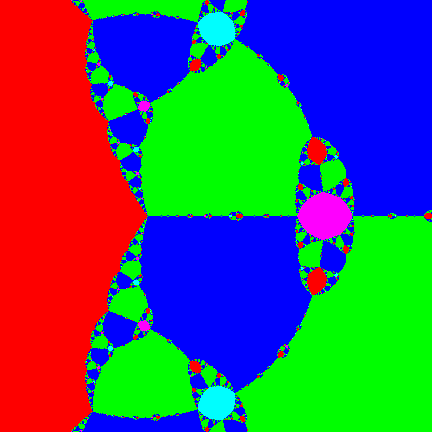
\includegraphics[width=0.23\textwidth]{../images/newton_div101.png}
  \end{center}
\end{frame}

\begin{frame}{Backup: limitations \& what I'd do differently}
  % TODO(tona): this needs your own voice, not mine — I've only
  % populated it with genuine open questions pulled from the source
  % (chapters/5-closing/closing.tex and the infinitary-amoebas open
  % questions section), which are legitimate but not the same thing as
  % a reflective "what I'd do differently." Please edit/replace.
  \begin{itemize}
    \item Dichromatic number: the Raghavan--Xiao basis for the uncountable directed threshold is size $\mathfrak c$, unknown whether that's optimal, or whether restricting to structurally simpler digraph classes helps.
    \item \tFer group: the infinitary theory currently only has trees; characterizing local amoebas among general countably infinite graphs is open, as is the Borel complexity of the local-amoeba property itself.
    \item Genuinely rigid graphs: checked up to 7 vertices; no structural (forbidden-subgraph-style) proof strategy yet in view.
  \end{itemize}
\end{frame}
\fi

\end{document}
